\documentclass[11pt]{article}

\usepackage[utf8]{inputenc}
\usepackage[margin=1in]{geometry}  % Adjust page margins
\usepackage{graphicx}              % For including images (PDF, PNG, JPG)
\usepackage[inkscapelatex=false]{svg}
\usepackage{listings}              % For including code
\usepackage{xcolor}                % For custom colors
\usepackage{hyperref}              % For hyperlinks in the PDF
\usepackage{amsmath, amssymb, amsthm} % For math symbols and environments
\usepackage{mathrsfs}
\usepackage{enumitem}
\geometry{a4paper, margin=1in} % Set margin to 1 inch
\usepackage{fancyhdr} % For header and footer
\usepackage{hyperref} % For clickable links in the PDF
\usepackage{array} % For table column formatting
\usepackage{times} % Uses Times font for the text
\usepackage{float}
\usepackage{multirow}
\usepackage{booktabs}


\title{CMOR 421/521 Assignment 3: Using MPI to implement Cannon's algorithm and SUMMA algorithm}
\author{Yuhao Liu}
\date{\today}

% --------------------------------------------------------------------------------
% Customize the appearance of code listings (for C++ syntax).
% --------------------------------------------------------------------------------
\lstdefinestyle{C++Style}{
    language=C++,
    basicstyle=\small\ttfamily,
    keywordstyle=\color{blue}\bfseries,
    commentstyle=\color{gray},
    stringstyle=\color{magenta},
    numbers=left,
    numberstyle=\tiny,
    stepnumber=1,
    breaklines=true,
    tabsize=4,
    showstringspaces=false
}

% If you store SVG images in a subfolder, specify the path here. 
% e.g.: \svgpath{{../images/}}
\svgpath{{./}}

\begin{document}

\maketitle

\tableofcontents
\bigskip

\newpage

\section{Directory Structure}
Below is my file organization for this assignment. 
My final zip file follows this structure ( \texttt{docs/} for LaTeX, \texttt{src/} for source files, and \texttt{include/} for header files):

\begin{figure}[H]
    \centering
    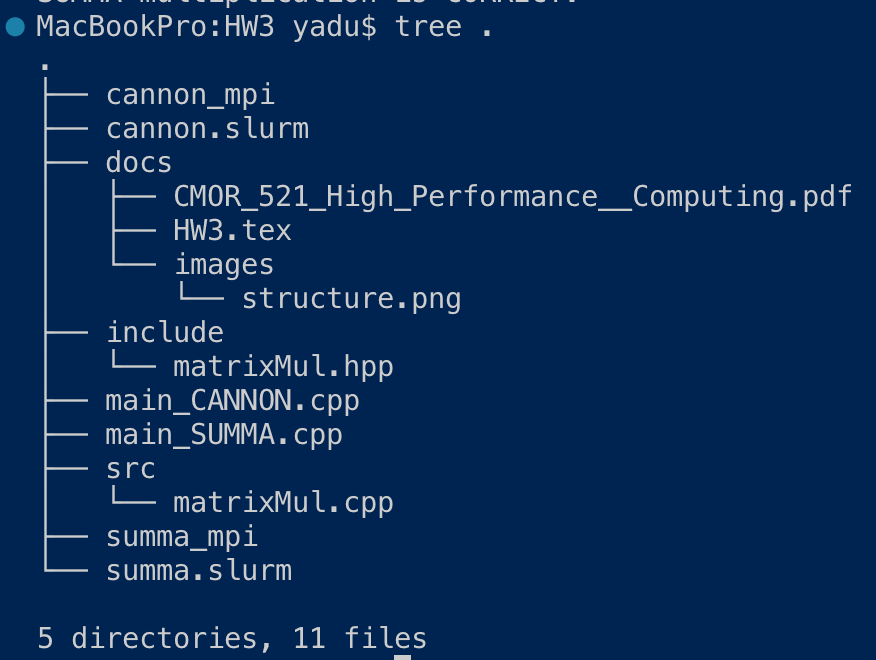
\includegraphics[width=0.5\linewidth]{Assignments/HW3/docs/images/structure.png}
    \caption{structure}
    \label{fig:structure}
\end{figure}

\begin{itemize}
    \item The \verb|include| folder and \verb|src| folder have \verb|matrixMul.hpp| and \verb|matrixMul.cpp|. In \verb|matrixMul.cpp|, there are 2 help function 
    \begin{itemize}
        \item \texttt{void testMul(const int N, double* serialC, double* mpiC);}  
    
        \item \texttt{void serialMatMult(const int N, double* C, const double* A, const double* B);}  
    \end{itemize}

    \item The \verb|main_CANNON.cpp| and \verb|main_SUMMA.cpp| contain the Cannon's algorithm and SUMMA algorithm respectively.
    \item The \verb|cannon_mpi| and \verb|summa_mpi| are executable files. Both of them already complied by \verb|-O3| optimization flag.
    \item The \verb|cannon.slurm| and \verb|summa.slurm| are sbatch scripts.
\end{itemize}

\newpage

\section{How to Build and Run the Code (In NOTXs)}
\begin{itemize}
    \item \textbf{Build and run}
        \begin{itemize}
            \item For each algorithm you can using
            \begin{verbatim}
                sbatch summa.slurm
                sbatch cannon.slurm
            \end{verbatim}
            to run these 2 different algorithm with $2 \times 2$, $3 \times 3$, $4 \times 4$ grids with $N = 512, 768, 1024$ and $k = 64$. All configuration parameters are defined in the \verb|*.slurm| job submission script. The following example illustrates the contents of \verb|summa.slurm| used for executing the SUMMA algorithm:

\begin{verbatim}
#!/bin/bash
#SBATCH --job-name=SUMMA
#SBATCH --account=commons
#SBATCH --partition=commons
#SBATCH --ntasks=16             # Total number of MPI processes
#SBATCH --cpus-per-task=1       # One CPU core per MPI process
#SBATCH --mem-per-cpu=16000     # Memory per core (in MB)
#SBATCH --time=00:30:00         # Walltime limit
#SBATCH --mail-user=yl336@rice.edu
#SBATCH --mail-type=END,FAIL

echo "Job running on nodes: $SLURM_NODELIST"
echo "================================================="

# Change to working directory
cd /home/yl336/cmor521/CMOR-521-High-Performance-Computing/Assignments/HW3 || exit

# Load compiler and MPI module
module load GCC/13.2.0
module load OpenMPI/4.1.6

# Compile the SUMMA program
mpic++ -O3 -o summa_mpi main_SUMMA.cpp ./src/matrixMul.cpp

# Execute the program on different processor grids
echo "=== Running SUMMA on 4 procs (2×2 grid) ==="
mpirun -n 4  ./summa_mpi 512 64

echo "=== Running SUMMA on 9 procs (3×3 grid) ==="
mpirun -n 9  ./summa_mpi 768 64

echo "=== Running SUMMA on 16 procs (4×4 grid) ==="
mpirun -n 16 ./summa_mpi 1024 64

echo "All runs complete."
\end{verbatim}

        \end{itemize}
\item \textbf{Results:}
\begin{itemize}
    \item \textbf{SUMMA Algorithm}
    \begin{itemize}
        \item \textbf{4 processes (2×2 grid)}  
              \begin{itemize}
                  \item Matrix size: 512
                  \item SUMMA time: \texttt{0.0419424} seconds
                  \item Serial time: \texttt{0.337914} seconds
                  \item Total error: \texttt{1.55078e-08}
                  \item Status: \texttt{CORRECT}
              \end{itemize}
        \item \textbf{9 processes (3×3 grid)}  
              \begin{itemize}
                  \item Matrix size: 768
                  \item SUMMA time: \texttt{0.084537} seconds
                  \item Serial time: \texttt{0.861577} seconds
                  \item Total error: \texttt{7.07854e-08}
                  \item Status: \texttt{CORRECT}
              \end{itemize}
        \item \textbf{16 processes (4×4 grid)}  
              \begin{itemize}
                  \item Matrix size: 1024
                  \item SUMMA time: \texttt{0.0979639} seconds
                  \item Serial time: \texttt{7.28481} seconds
                  \item Total error: \texttt{1.72492e-07}
                  \item Status: \texttt{CORRECT}
              \end{itemize}
    \end{itemize}

    \item \textbf{Cannon's Algorithm}
    \begin{itemize}
        \item \textbf{4 processes (2×2 grid)}  
              \begin{itemize}
                  \item Matrix size: 512
                  \item Cannon time: \texttt{0.0235929} seconds
                  \item Serial time: \texttt{0.62207} seconds
                  \item Total error: \texttt{1.13176e-08}
                  \item Status: \texttt{CORRECT}
              \end{itemize}
        \item \textbf{9 processes (3×3 grid)}  
              \begin{itemize}
                  \item Matrix size: 768
                  \item Cannon time: \texttt{0.0345131} seconds
                  \item Serial time: \texttt{1.03666} seconds
                  \item Total error: \texttt{6.90086e-08}
                  \item Status: \texttt{CORRECT}
              \end{itemize}
        \item \textbf{16 processes (4×4 grid)}  
              \begin{itemize}
                  \item Matrix size: 1024
                  \item Cannon time: \texttt{0.039058} seconds
                  \item Serial time: \texttt{5.11798} seconds
                  \item Total error: \texttt{1.63165e-07}
                  \item Status: \texttt{CORRECT}
              \end{itemize}
    \end{itemize}
\end{itemize}

\end{itemize}
\end{document}